\documentclass{article}

\usepackage{amsmath, graphicx}

\title{Homework3 Report}
\author{Qi Liu}
\date{\today}

\begin{document}
	
\maketitle

\section{Hard Margin SVM}

\subsection{Perpendicular}
The boundary is a hyperplane $w^Tx+b=0$. For any two points $x_1, x_2$ in this hyperplane, we have $w^Tx_1+b=0$ and $w^Tx_2+b=0$. This implies $w^T(x_2-x_1)=0$ which means $w$ is perpendicular to the vector $\overrightarrow{x_1x_2}$. Due to $x_1$ and $x_2$ can be chosen arbitrarily, $w$ is perpendicular to any vector in the hyperplane. Thus $w$ is perpendicular to the hyperplane which is the boundary.

\subsection{Support Vectors}
Due to $x$ is the support vector of the positive class, we have $w^Tx+b=1$, then $b=1-w^Tx$. By the same method, $b=-1-w^Ty$ if $y$ is the support vector of the negative class.

\subsection{Linear Boundary}
\begin{center}
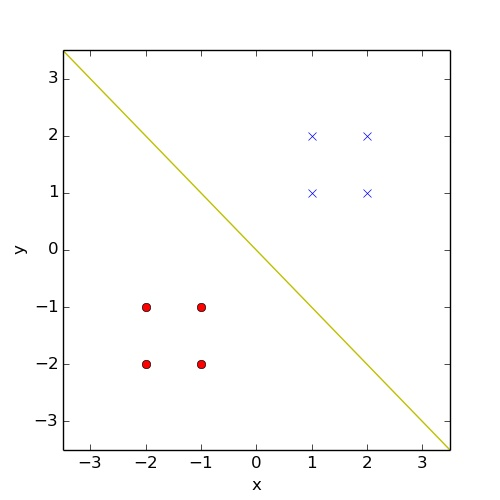
\includegraphics[width=0.5\textwidth]{../result/linear_boundary.jpg}
\end{center}
The boundary is shown as the yellow line in the above figure. The two support vectors are $(-1,-1)$ and $(1, 1)$.

\subsection{Circular Boundary}
\begin{center}
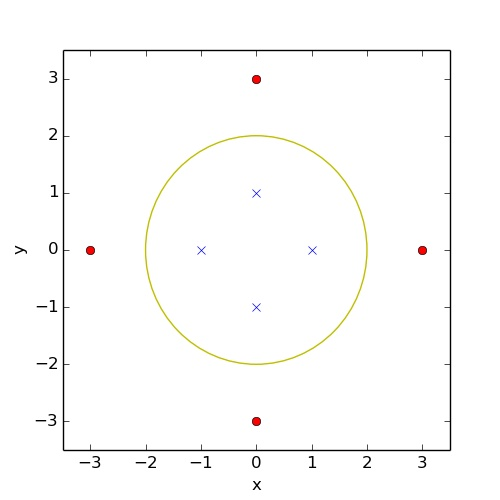
\includegraphics[width=0.5\textwidth]{../result/circular_boundary.jpg}
\end{center}
The boundary is shown as the yellow circle in the above figure. We use the transform $\phi(x)=|x|$ thus kernel is $K(x,x')=|x||x'|$. For all positive samples, $\phi(x)=3$. For all negative samples, $\phi(x)=1$. Therefore the boundary is $\phi(x)=2$ which is just the yellow circle.

\section{Soft Margin SVM}
\end{document}